\begin{figure}[htp]
	\begin{center}
	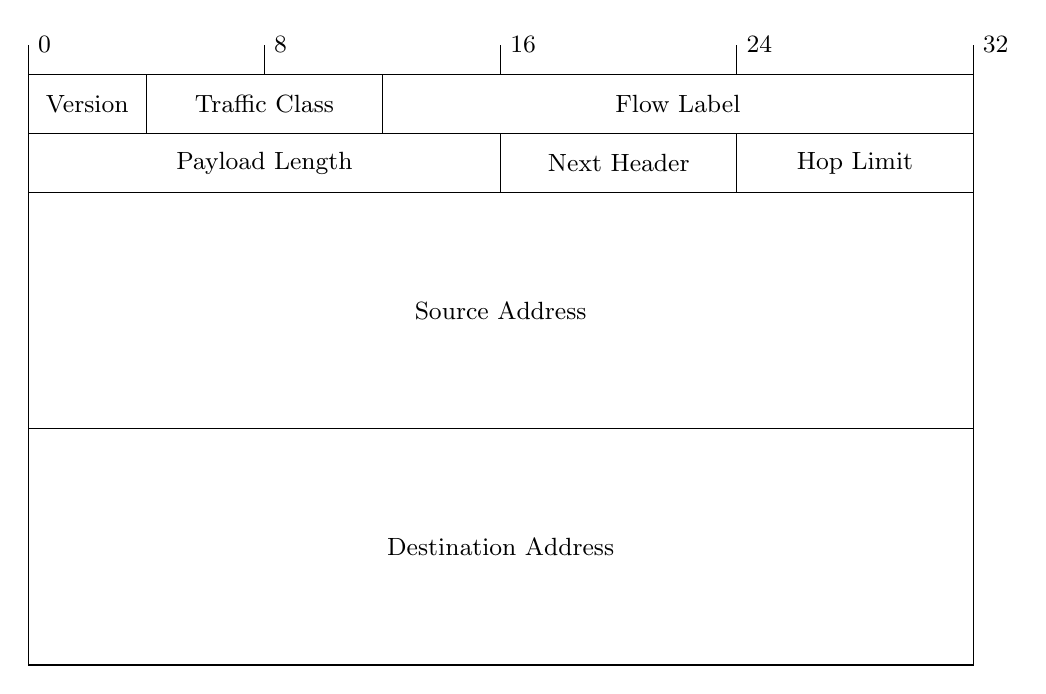
\begin{tikzpicture}[scale=0.75]
		\draw (0,0) -- (16,0) -- (16,10) -- (0,10) -- cycle;
		\draw (0,9) -- (16,9);
		\draw (0,8) -- (16,8);
		\draw (0,4) -- (16,4);
		\draw (0,10) -- ++(0,0.5) node[right] {\small 0};
		\draw (4,10) -- ++(0,0.5) node[right] {\small 8};
		\draw (8,10) -- ++(0,0.5) node[right] {\small 16};
		\draw (12,10) -- ++(0,0.5) node[right] {\small 24};
		\draw (16,10) -- ++(0,0.5) node[right] {\small 32};

		\draw (2,10) -- (2,9);
		\node at (1,9.5) {\small Version};
		\draw (6,10) -- (6,9);
		\node at (4, 9.5) {\small Traffic Class};
		\node at (11, 9.5) {\small Flow Label};

		\draw (8,9) -- (8,8);
		\node at (4, 8.5) {\small Payload Length};
		\draw (12,9) -- (12,8);
		\node at (10, 8.5) {\small Next Header};
		\node at (14,8.5) {\small Hop Limit};

		\node at (8, 6) {\small Source Address};
		\node at (8, 2) {\small Destination Address};
	\end{tikzpicture}
	\end{center}
	\caption{IPv6 Header}
	\label{fig:ipv6_hdr}
\end{figure}